\section{Introduction}
Long-horizon manipulation is commonly addressed by decomposing a task into subtasks with associated skills~\cite{konidaris2018skills,dalal2024manipgen,Ahn2022DoAI,merging_dmp}, each learned via reinforcement or imitation learning. Yet real-world execution introduces physical perturbations that can induce \emph{task-level} failures even when the low-level motion policy executes flawlessly. Consider a robot scooping rice from a bowl, transporting it, and depositing it onto a plate: an external disturbance that jostles the arm mid-transport merely deflects the path, from which a dynamical-systems-based movement primitive~\cite{Ijspeert_NC_2013,figueroa2018lpvds,DSbook} can spatially recover; but a disturbance that tips the spoon and slides the rice off is a \emph{task-level} failure: the arm still reaches the deposit location, on schedule, carrying nothing. Reaching the target does not resolve it. Robust manipulation therefore demands reactivity at both the motion \emph{and} the task level.

We adopt the well-established view that task-level reactivity is naturally expressed as a \emph{hybrid automaton}~\cite{burridge1999sequential,kressgazit2009temporal}: the joint robot--environment state space is partitioned into discrete \emph{modes} (here, \textit{Scoop}, \textit{Transport}, \textit{Deposit}), each mode selecting an active skill, with transitions governing the sequencing. Two properties make such an automaton robust to perturbation. \emph{Goal reachability} ensures each skill drives the state to the next transition boundary, guaranteeing task progress; \emph{mode invariance} ensures the state remains within a mode until that boundary (e.g., that the rice remains loaded on the spoon throughout \textit{Transport}), so that an unexpected departure from a mode is precisely a task-level failure signal. Temporal-logic imitation (TLI)~\cite{wang2022temporal} makes these conditions explicit and, when they hold for the learned per-mode policies, guarantees that any admissible discrete plan is realized by the continuous system.

\begin{figure}[t!]
\centering
% New positioning figure: the task automaton is SHARED; only how the localization
% function L is obtained differs across TLI (hand-designed), GLiDE (learned via
% perturb+reset+oracle), and SEAL (learned from safe segmented demos).
\resizebox{\columnwidth}{!}{%
\begin{tikzpicture}[>=Latex, font=\small,
  mode/.style={circle, draw, thick, minimum size=7.5mm, inner sep=0pt},
]
% ---------- Top: the shared, designed automaton ----------
\node[mode] (a) {$a$};
\node[mode, right=12mm of a] (b) {$b$};
\node[mode, right=12mm of b] (c) {$c$};
\node[mode, right=12mm of c, double, double distance=1pt] (d) {$d$};
\node[above=0pt of a, font=\scriptsize] {Scoop};
\node[above=0pt of b, font=\scriptsize] {Transport};
\node[above=0pt of c, font=\scriptsize] {Deposit};
\node[above=0pt of d, font=\scriptsize] {Done};
\draw[->,thick] (a) -- (b);
\draw[->,thick] (b) -- (c);
\draw[->,thick] (c) -- (d);
\draw[->, thick, red] (b) to[bend left=48] node[below=0.5pt, midway, font=\tiny, red] {recovery} (a);
\begin{scope}[on background layer]
  \node[draw, dashed, rounded corners, inner xsep=4.5mm, inner ysep=6mm, fit=(a)(b)(c)(d)] (auto) {};
\end{scope}
\node[anchor=west, font=\bfseries\small] at ([yshift=1mm]auto.north west)
  {Designed task automaton \normalfont(shared by all three methods)};
\node[font=\scriptsize\itshape, below=0.5mm of auto.south]
  {reactivity $=$ localizing the state onto the correct mode: where is the guard?};

% ---------- Bottom: the SAME guard, obtained three ways ----------
% Panel geometry: width 3.5, height 2.7. True guard: load falls as tilt grows.
% Macro-ish: draw each panel in a shifted scope.
%
% ---- Panel 1: TLI (hand-placed thresholds, no data) ----
\begin{scope}[shift={(-1.35,-4.6)}]
  \draw[->] (0,0) -- (3.5,0) node[below left, font=\tiny] {tilt $\theta$};
  \draw[->] (0,0) -- (0,2.7) node[rotate=90, anchor=south east, font=\tiny] {load $F$};
  % true boundary (unknown to the designer)
  \draw[gray!70, thick, dashed]
    (0.25,2.15) .. controls (1.4,1.95) and (2.1,1.15) .. (3.2,0.55);
  \node[gray!70, font=\tiny, anchor=west] at (0.30,2.38) {true guard};
  % hand-placed axis-aligned thresholds
  \draw[tli, very thick] (1.6,0) -- (1.6,1.0) -- (3.3,1.0);
  \node[tli, font=\tiny, anchor=west] at (1.62,0.32) {$\theta\!>\!20^{\circ}$};
  \node[tli, font=\tiny, anchor=south west] at (2.35,1.02) {$F\!<\!0.5$N};
  % mismatch region
  \begin{scope}[on background layer]
    \fill[red!14] (1.6,1.0) -- (1.6,1.83) .. controls (2.0,1.5) and (2.4,1.2)
      .. (2.75,1.0) -- cycle;
  \end{scope}
  \node[red!70, font=\tiny, anchor=west] at (2.15,1.95) {mismatch:};
  \node[red!70, font=\tiny, anchor=west] at (2.15,1.70) {missed failures};
  % region labels: above the guard rice is retained, below it is lost
  \node[gray, font=\tiny\itshape, anchor=west] at (2.30,2.45) {$R_{\text{transport}}$: rice on};
  \node[gray, font=\tiny\itshape] at (0.85,0.40) {rice lost $\to$ Scoop};
  \node[font=\scriptsize\bfseries, tli, anchor=north] at (1.75,-0.42) {\faDraftingCompass~TLI: hand-placed};
  \node[font=\tiny, tli, anchor=north] at (1.75,-0.82) {no data consulted};
\end{scope}
%
% ---- Panel 2: GLiDE (fit to induced failures) ----
\begin{scope}[shift={(3.05,-4.6)}]
  \draw[->] (0,0) -- (3.5,0) node[below left, font=\tiny] {tilt $\theta$};
  \draw[->] (0,0) -- (0,2.7);
  % failure cloud (below/right of true boundary)
  \foreach \p in {(1.9,0.6),(2.3,0.85),(2.7,0.5),(2.5,1.0),(3.0,0.75),(2.1,0.35),
                  (2.85,0.32),(1.75,0.95),(2.45,0.6),(3.1,1.0),(2.05,1.12),(2.65,1.28)}
    \node[red!75, font=\tiny] at \p {$\times$};
  % success cloud (above/left)
  \foreach \p in {(0.5,1.7),(0.9,2.1),(1.3,1.75),(0.6,2.35),(1.6,1.6),(1.05,1.45),
                  (1.5,2.2),(0.35,1.35),(1.85,1.75),(0.85,1.75)}
    \fill[glide] \p circle (1.3pt);
  % fitted boundary hugs the truth
  \draw[glide, very thick]
    (0.25,2.15) .. controls (1.4,1.95) and (2.1,1.15) .. (3.2,0.55);
  % region labels + oracle legend
  \node[gray, font=\tiny\itshape, anchor=west] at (2.30,2.45) {rice on};
  \node[gray, font=\tiny\itshape] at (0.85,0.40) {rice lost};
  \node[glide, font=\tiny, anchor=west] at (0.15,0.15)
    {$\bullet$ valid\ \ \textcolor{red!75}{$\times$} invalid transition (oracle)};
  \node[font=\scriptsize\bfseries, glide, anchor=north] at (1.75,-0.42) {\faExclamationTriangle~GLiDE: fit to failure};
  \node[font=\tiny, glide, anchor=north] at (1.75,-0.82) {$1000$s of spills \faRedo\ resets + oracle};
\end{scope}
%
% ---- Panel 3: SEAL (fit to success only) ----
\begin{scope}[shift={(7.45,-4.6)}]
  \draw[->] (0,0) -- (3.5,0) node[below left, font=\tiny] {tilt $\theta$};
  \draw[->] (0,0) -- (0,2.7);
  % a few safe demonstration trajectories (stay on the safe side of the guard)
  \draw[seal!70, thick] (0.35,2.45) .. controls (1.0,2.5) and (1.5,2.15) .. (1.9,1.70);
  \draw[seal!70, thick] (0.5,2.25) .. controls (1.2,2.30) and (1.7,1.85) .. (2.2,1.45);
  \draw[seal!70, thick] (0.6,2.60) .. controls (1.5,2.55) and (2.0,1.85) .. (2.5,1.35);
  % query points proposed by the GPC at its most uncertain guard states
  \foreach \p in {(2.9,0.82),(2.55,1.08),(3.05,0.74)}{
    \fill[seal] \p circle (1.5pt);
    \draw[seal] \p circle (3.0pt);
  }
  \node[seal, font=\tiny, anchor=south west] at (2.55,1.55) {queries};
  % newly requested SAFE demos passing through the queried states (dashed)
  \draw[seal!70, thick, dashed] (2.05,1.65) .. controls (2.35,1.30) .. (2.55,1.08)
    .. controls (2.75,0.90) .. (3.05,0.74);
  \draw[seal!70, thick, dashed] (2.45,1.45) .. controls (2.70,1.10) .. (2.9,0.82)
    .. controls (3.00,0.73) .. (3.12,0.66);
  % region labels
  \node[gray, font=\tiny\itshape, anchor=east] at (3.35,2.20) {rice on};
  \node[gray, font=\tiny\itshape] at (0.85,0.40) {rice lost};
  % fitted boundary hugs the truth
  \draw[seal, very thick]
    (0.25,2.15) .. controls (1.4,1.95) and (2.1,1.15) .. (3.2,0.55);
  \node[font=\scriptsize\bfseries, seal, anchor=north] at (1.75,-0.42) {\faIcon{shield-alt}~SEAL: fit to success};
  \node[font=\tiny, seal, anchor=north] at (1.75,-0.82) {few safe demos + targeted queries};
\end{scope}
%
% connective tissue: all three feed the same L
\node[font=\scriptsize\itshape] at (4.8,-6.9)
  {three ways to obtain the same object: the localization function $L:\ \mathcal{X}_{\min}\!\to\!\mathcal{M}$};
\end{tikzpicture}%
}

\caption{\textbf{One automaton, one guard, three ways to find it.} \emph{Top:} all methods share the same designed automaton for scooping; reactivity reduces to knowing where the \emph{guard} lies in feature space (spoon tilt $\theta$ vs.\ load $F$). In each bottom panel the dark curve is that guard, separating \textit{Transport} still valid (rice on) from physically failed (rice lost $\to$ re-localize to \textit{Scoop}). TLI~\cite{wang2022temporal} places it by hand: where the analytic rule and the true boundary disagree (shaded), failures go undetected and no data corrects it. GLiDE~\cite{wang2024grounding} fits it to perturbed rollouts labeled by an outcome oracle: accurate, but at the cost of thousands of induced failures and resets. SEAL fits it from a few safe demonstrations (solid) plus safe demonstrations queried at its most uncertain states (circled, dashed); no failure is ever induced.}
\label{fig:seal_ltl_comp}
\end{figure}
\begin{figure*}[t!]
\centering
% TikZ scaffold + photo frames. Photos in Figures/intro_frames/ are LOW-RES CROPS of
% the old simple.png -- replace each file with the original high-res photo (same
% filename) and the figure updates automatically.
\resizebox{\textwidth}{!}{%
\begin{tikzpicture}[font=\small,
  photo/.style={inner sep=0pt, outer sep=0pt},
  quote/.style={font=\scriptsize\itshape, text depth=0pt},
  banner/.style={font=\small\bfseries, anchor=west},
]
% ---------- (1) Teach ----------
\node[photo] (t1) {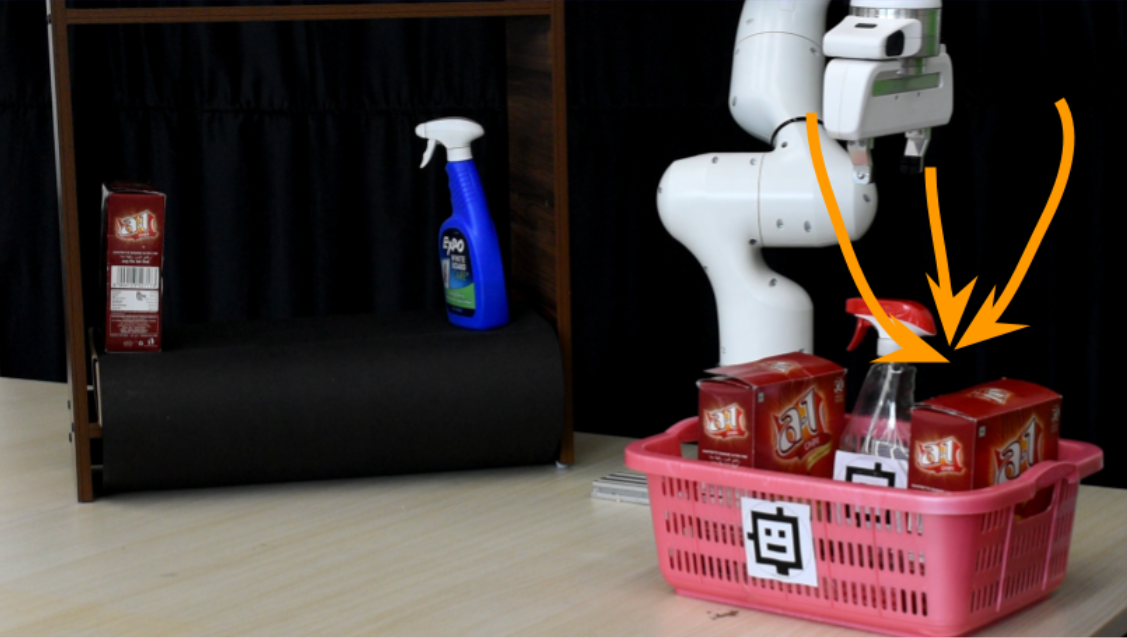
\includegraphics[width=3.1cm]{Figures/intro_frames/teach1.png}};
\node[photo, right=1.5mm of t1] (t2) {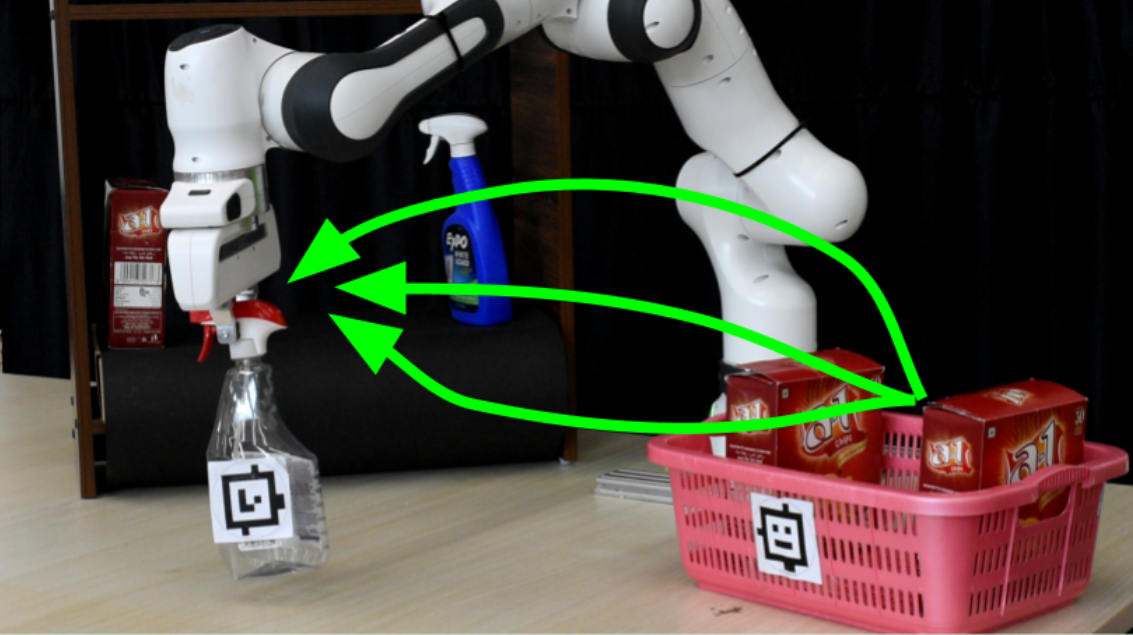
\includegraphics[width=3.1cm]{Figures/intro_frames/teach2.png}};
\node[photo, right=1.5mm of t2] (t3) {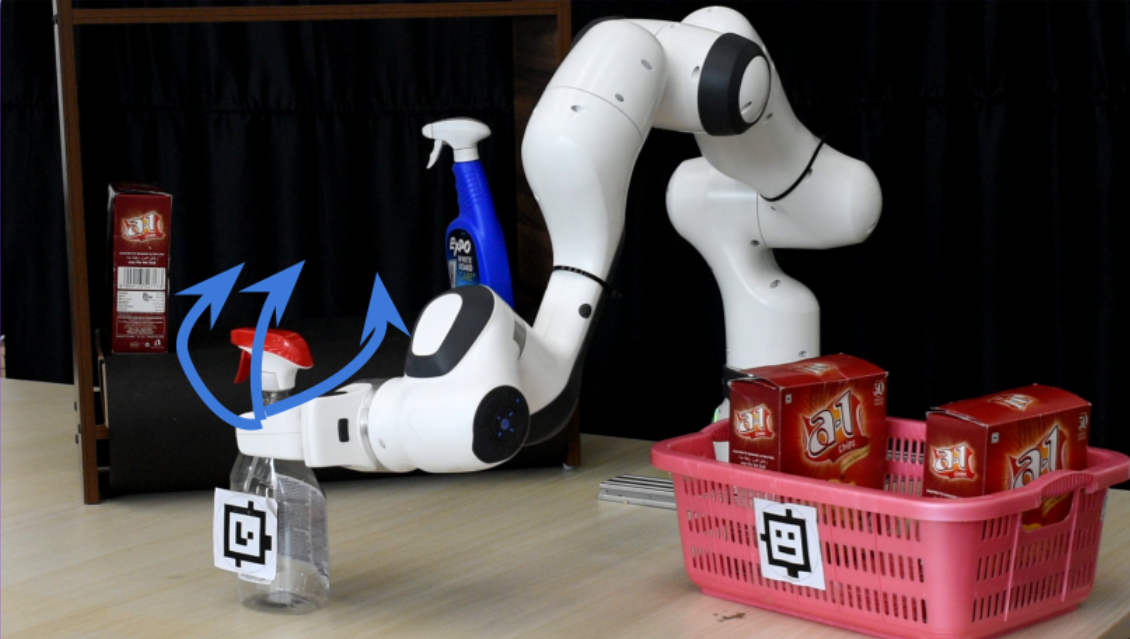
\includegraphics[width=3.1cm]{Figures/intro_frames/teach3.png}};
\node[photo, right=1.5mm of t3] (t4) {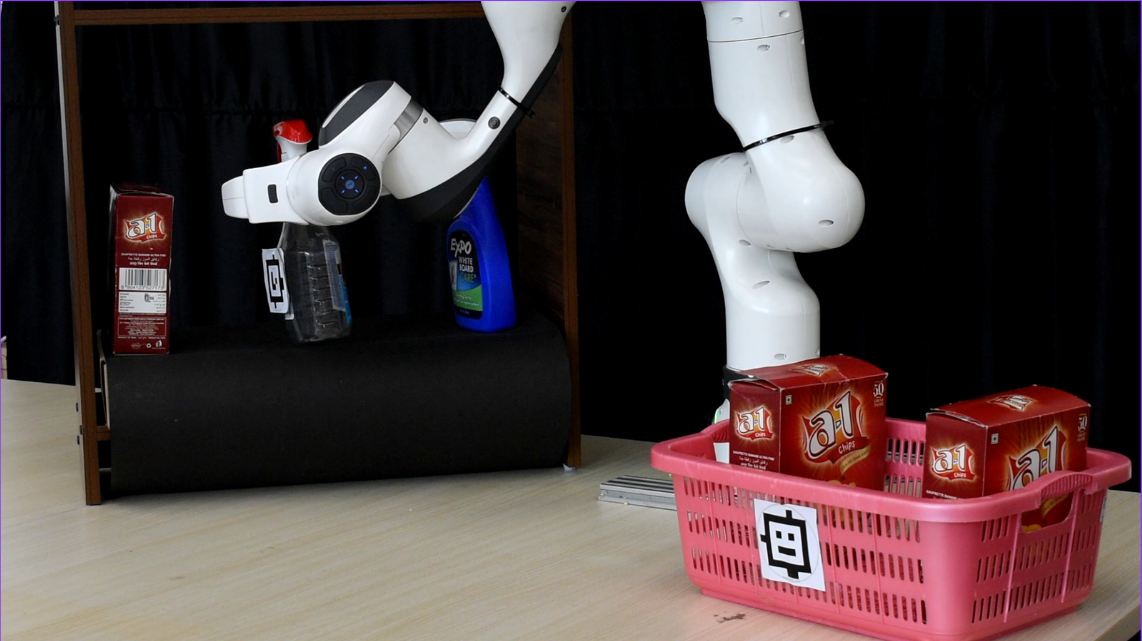
\includegraphics[width=3.1cm]{Figures/intro_frames/teach4.png}};
\node[quote, below=0.5mm of t1] {``grasping from top''};
\node[quote, below=0.5mm of t2] {``placing on table''};
\node[quote, below=0.5mm of t3] {``grasping from side''};
\node[quote, below=0.5mm of t4] {``placing on shelf''};
\node[banner, tli] at ([xshift=-1mm,yshift=3.5mm]t1.north west)
  {\faUser~1.\ Expert teaches: narrated, segmented demonstrations};
\begin{scope}[on background layer]
  \node[fill=teachbg, rounded corners, inner sep=2.5mm,
        fit=(t1)(t4), yshift=-1mm, minimum height=2.6cm] (teachbox) {};
\end{scope}
% ---------- (2) Query ----------
\node[photo, below=13mm of t1.south west, anchor=north west] (q1a)
  {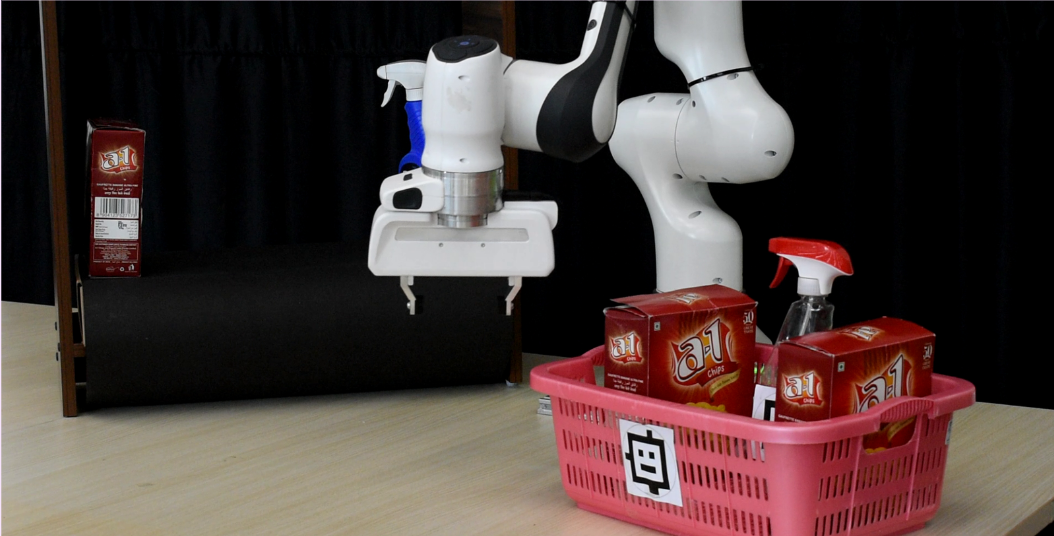
\includegraphics[width=2.75cm]{Figures/intro_frames/query1a.png}};
\node[photo, right=4mm of q1a] (q1b) {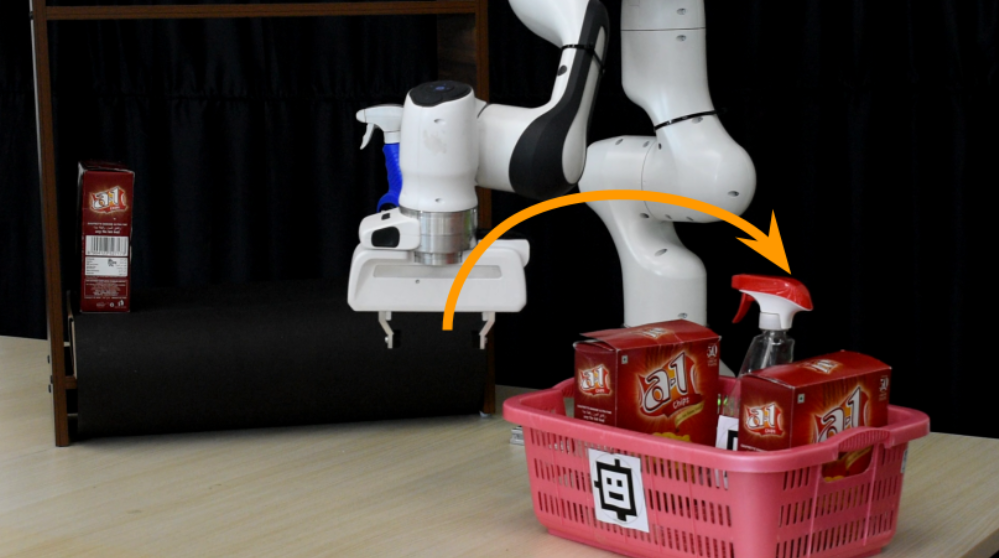
\includegraphics[width=2.75cm]{Figures/intro_frames/query1b.png}};
\node[photo, right=7mm of q1b] (q2a) {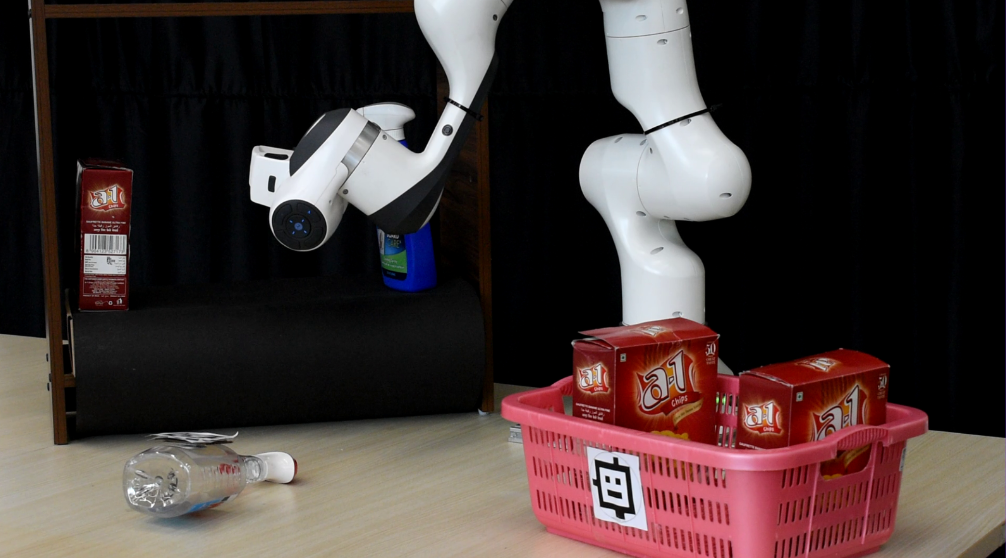
\includegraphics[width=2.75cm]{Figures/intro_frames/query2a.png}};
\node[photo, right=4mm of q2a] (q2b) {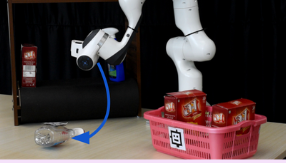
\includegraphics[width=2.75cm]{Figures/intro_frames/query2b.png}};
\draw[->, thick] (q1a) -- (q1b);
\draw[->, thick] (q2a) -- (q2b);
\node[quote, below=0.5mm of q1b.south west, anchor=north] at ([xshift=-3mm]q1b.south west|-q1b.south)
  {};
\node[quote] at ([yshift=-2.5mm]$(q1a.south)!0.5!(q1b.south)$) {\faUser~``I would grasp from top''};
\node[quote] at ([yshift=-2.5mm]$(q2a.south)!0.5!(q2b.south)$) {\faUser~``I would grasp from side''};
\node[banner, tli] at ([xshift=-1mm,yshift=3.5mm]q1a.north west)
  {\faRobot~2.\ Robot queries the situations it is uncertain about};
\begin{scope}[on background layer]
  \node[fill=querybg, rounded corners, inner sep=2.5mm,
        fit=(q1a)(q2b), yshift=-1mm, minimum height=2.6cm] (querybox) {};
\end{scope}
% ---------- (3) Test ----------
\node[photo, right=8mm of t4.north east, anchor=north west, yshift=-9mm] (test)
  {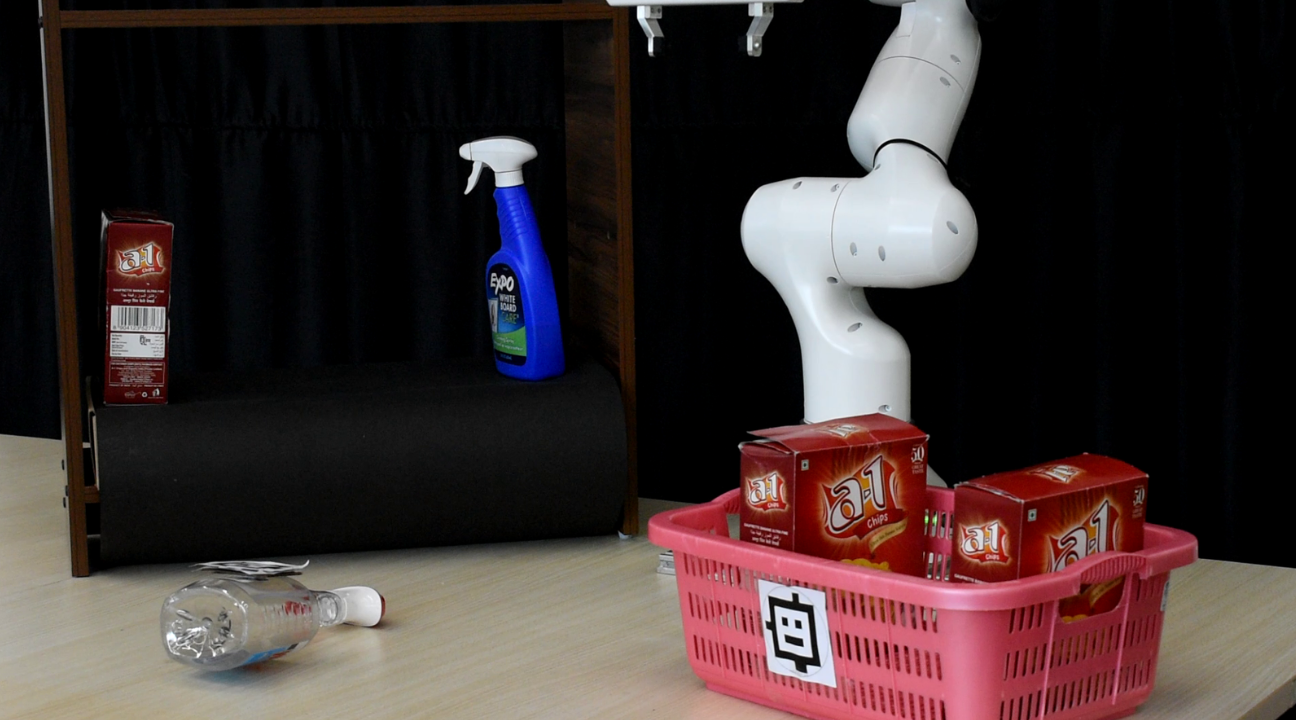
\includegraphics[width=4.1cm]{Figures/intro_frames/test.png}};
\node[banner, tli, text width=4.1cm, align=left] at ([xshift=-1mm,yshift=6mm]test.north west)
  {\faBolt~3.\ Test: perturbation};
\node[font=\scriptsize, align=center, below=1.5mm of test]
  (testtxt) {bottle knocked over $\rightarrow$ localizer\\ detects mode change $\rightarrow$\\ ``grasp from side'' engaged\\ \textbf{failure avoided}};
\begin{scope}[on background layer]
  \node[fill=testbg, rounded corners, inner sep=2.5mm, fit=(test)(testtxt)] {};
\end{scope}
\end{tikzpicture}%
}

\caption{\textbf{Teaching, querying, and recovery on the restocking task.} (1) The expert demonstrates the full task, marking each subtask with a trigger signal while narrating. (2) The trained classifier identifies the physical situations where its guard estimate is most uncertain and asks the expert what mode should be executed from them; the answers are short, safe sub-demonstrations. (3) At test time the memory-less localizer detects a perturbation-induced mode change from the instantaneous state and engages the appropriate skill.}
\label{fig:intro}
\end{figure*}

Crucially, in this formalism the discrete modes are only labels; the semantic content and the robustness both reside in the \emph{transitions} and in the function that grounds continuous state to modes. We call this the \emph{localization function} $L:\mathcal{X}\!\to\!\mathcal{M}$. For our scooping robot, $L$ must decide, from signals such as the spoon-tilt angle and a contact/load reading, which of $\{$\textit{Scoop}, \textit{Transport}, \textit{Deposit}$\}$ is currently active and, implicitly, exactly where the boundary between them, the \emph{guard}, lies in that feature space. Given the automaton, runtime reactivity reduces entirely to this: localize the current state onto the correct side of the guard, at every control step. The automaton itself is easy to write down; the guard is where the difficulty lives. The central question of this paper is therefore \emph{how the guard is obtained}, and at what cost in expertise, data, and safety (Fig.~\ref{fig:seal_ltl_comp}).

The classical answer, exemplified by TLI, is to place the guard by hand (Fig.~\ref{fig:seal_ltl_comp}, bottom left): an expert authors it analytically, reasoning from a physical model of the task (rice mass, spoon geometry, expected sensor range) to a rule such as ``a load reading below 0.5\,N while tilt exceeds $20^\circ$ means \textit{Transport} has failed.'' This consumes no data at all; the guard is placed by expertise alone, and its accuracy is bounded by how well the expert's analytic model matches the true sensor and task distribution. If real load-cell noise, rice clumping, or spoon-to-grain friction deviate from that model, as they generally do, the guard is simply in the wrong place, and no amount of subsequent operation corrects it, because no data was ever consulted in placing it. Hand-designed grounding is thus brittle to observation noise (Sec.~\ref{sec:scooping}) not for lack of engineering effort, but by construction.

\textbf{REBUTTAL: I think reducing TLI to just hand defined modes might be seen unfavourably. It hand-designs some sensors but also uses failures to transfer those boundaries to the robot space. I think we can have 4 examples - the first one will be standard hand designed modes. The second will be TLI, he third GLIDE and the fourth SEAL.}

GLiDE~\cite{wang2024grounding} recognizes exactly this mismatch and fits the guard to data instead of asserting it (Fig.~\ref{fig:seal_ltl_comp}, bottom center). It perturbs demonstrations (tilting the spoon further, jostling the arm), replays them, and uses an automatic success/failure oracle together with a reset mechanism to label thousands of rollouts, then fits the mode boundaries to the resulting cloud of successes and failures. The guard now hugs the real distribution rather than an idealized model of it. But tracing the boundary this way requires \emph{inducing} the failure, repeatedly and at volume: to learn where rice falls off the spoon, GLiDE must spill rice, thousands of times, in an environment that can automatically detect the spill and reset it. For contact-rich tasks this is precisely the regime that does not exist: grains cannot be un-spilled, payloads cannot be un-dropped, and a deployed system exists to avoid these outcomes, not to rehearse them.

The two state-of-the-art answers thus sit at uncomfortable extremes: TLI needs no data but inherits every error of the expert's analytic model, while GLiDE fixes the model error only by consuming failure data that is unsafe, expensive, or physically impossible to collect. What is missing is a way to fit the guard to the \emph{real} distribution, retaining GLiDE's data-driven accuracy, while using only data that is safe to produce. This is the gap SEAL fills: a handful of safe, human-segmented demonstrations gives an initial estimate of the guard, and a small number of additional safe demonstrations, actively requested at the specific states where that estimate is least certain, sharpen it to the precision that would otherwise demand a cloud of failures (Fig.~\ref{fig:seal_ltl_comp}, bottom right; pipeline in Fig.~\ref{fig:intro}). No rice is ever spilled to learn where it would spill.

\textbf{Approach.} SEAL retains the designed automaton and learns its localization function, never requiring resets, self-supervised rollouts, or failure data. An LLM proposes a compact set of spatially invariant features from the task description, and an information-theoretic check certifies that the modes are actually separable in that space before any learning begins. A Gaussian Process Classifier trained on the segmented demonstrations then serves as the localizer; its epistemic uncertainty pinpoints the states at which the guard estimate is weakest, and these states become the active demonstration requests. At runtime the localizer reads the instantaneous physical state (the current tilt and load reading, not the history of modes visited), so a perturbation that drives the state across a mode boundary is registered within a control step and recovery is triggered, regardless of where the nominal plan believes the task to be. By thresholding the classifier's predictive confidence, transitions are accepted only when confident and persistent, decoupling switching latency from the false-positive rate.



\textbf{Contributions.}
\begin{enumerate}
\item \textbf{Safe localization from success-only demonstrations.} We formulate reactive sequencing as learning the localization function of a known automaton from safe data alone, and provide a two-stage feature-engineering pipeline that pairs an LLM semantic prior with an information-theoretic \emph{observability certificate}, yielding a minimal, spatially invariant space in which modes are instantaneously separable.
\item \textbf{Uncertainty-targeted active querying.} A Gaussian Process Classifier exposes epistemic uncertainty that directs expert effort to under-determined guard regions (without perturbations, resets, or failure data), and the same signal extends naturally to invariance/reachability-driven guard refinement against the true closed-loop dynamics.
\item \textbf{Confidence-gated switching.} We exploit the classifier's predictive confidence to achieve low switching latency and a low false-positive rate simultaneously: a trade-off that hand-tuned automata and uncalibrated groundings must instead resolve with long debounce windows.
\item \textbf{Extensive validation} across five simulated and real-world contact-rich tasks and a 10-participant user study, including an empirical certification of goal reachability and mode invariance on the learned regions.
\end{enumerate}

%%%%%%%%%%%%%%%%%%%%%%%%%%%%%%%%%%%%%%%%%%%%%%%%%%%%%%%%%%%%%%%%%%%%%%%%%%%%%%%%
